\documentclass[12pt]{report}
\usepackage{mathptmx}		% font
\usepackage[a4paper,top=15mm, bottom=25mm, left=23mm, right=23mm]{geometry} % geometry/margins of page
\usepackage[lastpage,user]{zref}
\usepackage[english]{babel}
\usepackage[usenames, dvipsnames]{color}
\usepackage{setspace}

\usepackage{fancyhdr}
\usepackage{graphicx}
\usepackage{hyperref}
\usepackage{array}
\usepackage[utf8]{inputenc}
\usepackage{titlesec}
\usepackage{fixltx2e}
\usepackage{amssymb}
\usepackage{tikz}
\usepackage{multirow}
\usepackage{tabularx}
\pagestyle{fancy}

\setlength{\parindent}{0pt}	% no paragraph indentation
\setcounter{secnumdepth}{0}
\addto\captionsenglish{% Replace "english" with the language you use
  \renewcommand{\contentsname}%
    {Tartalomjegyz\'{e}k}%
}
\renewcommand{\headrulewidth}{0pt}
\newcommand{\mychapter}[2]{
    \setcounter{chapter}{#1}
    \setcounter{section}{0}
    \chapter*{#2}
    \addcontentsline{toc}{chapter}{#2}
}
\definecolor{BlueA}{RGB}{0, 69, 134}
\definecolor{BlueB}{RGB}{20, 39, 160}
\titleformat{\section}
{\color{BlueB}\normalfont\Large\bfseries}
{\color{BlueB}\thesection}{1em}{}
\titleformat{\subsection}
{\color{BlueA}\normalfont\Large\bfseries}
{\color{BlueA}\thesubsection}{1em}{}
\fancyhead{}
\DeclareGraphicsExtensions{.pdf,.png,.jpg}
\usetikzlibrary{arrows,shapes,positioning,shadows,trees}

\tikzset{
  basic/.style  = {draw, text width=2cm, drop shadow, font=\sffamily, rectangle},
  root/.style   = {basic, rounded corners=2pt, thin, align=center,
                   fill=blue!30},
  level 2/.style = {basic, rounded corners=6pt, thin,align=center, fill=blue!20,
                   text width=5em}
}

\cfoot{\thepage\ / \zpageref{LastPage}}

\begin{document}

\begin{center}				% center everything on the titlepage
\vspace*{100px}
\textcolor{BlueA}{	
{\fontsize{8mm}{8mm}\selectfont
	\textbf{Programoz\'{a}si alapismeretek\linebreak beadand\'{o} feladat}
	\vspace{4mm}
	\textbf{\linebreak T\"{o}rzsek: D, R, BB, TT}
	}
}
\vspace{40mm}				% vertical spacing

% subtitle 1
\textcolor{BlueA}{	
{\fontsize{14pt}{14pt}\selectfont
	\textbf{K\'{e}sz\'{i}tette: Lest\'{a}r Norbert\linebreak}
	\textbf{Neptun-azonosító: A8UZ7T \linebreak}
	\textbf{E-mail: \textcolor{blue}{\protect\href{mailto:lestarnrbert@inf.elte.hu}{lestarnrbert@inf.elte.hu}}}
	}
}

\vspace{15mm}

\textcolor{BlueA}{	
{\fontsize{14pt}{14pt}\selectfont
	\textbf{Kurzuskód: IP-08PAEG\linebreak}
	\textbf{Gyakorlatvezető neve: Nagy Sára}
	}
}

\vspace{40mm}

\textcolor{BlueA}{	
{\fontsize{18pt}{18pt}\selectfont
	\textbf{2014. november 20.}
	}
}

\vspace{7pt}				% vertical spacing	

\end{center}

\pagebreak
\tableofcontents

\pagebreak
\mychapter{0}{Felhaszn\'{a}l\'{o}i dokument\'{a}ci\'{o}}
\section{Feladat}
A jelenlegi Dél-Afrikai Köztársaság területén számos törzs élt, amikor a fehér gyarmatosítók
megjelentek. Közülük egyesek békében éltek, mások időről időre ellenséges viszonyba
keveredtek vagy éppen harcban álltak szomszédjaikkal. A háborúkat kezdőidő szerinti
sorrendben ismerjük a XVII., XVIII., XIX. századból.\newline

\vspace{1mm}

\begin{tabular}{rl}
\textbf{Sorszám} & \textbf{Feladat szövege} \\
D & Mennyi volt a háborúk átlagos ideje? \\
R & Volt békés törzs, és ha igen, akkor melyik? \\
BB & Melyik törzs háborúzott legtöbbször, és összesen mennyiszer? \\
TT & Volt egyszer hadba vonuló törzs, és ha igen, akkor melyik? \\
\end{tabular}
\section{Használat}
\subsection{A program indítása}
A program az A8UZ7T\_Torzsek/bin/Debug/A8UZ7T\_Torzsek.exe néven található a tömörített állományban. Az A8UZ7T\_Torzsek.exe fájl kiválasztásával indítható.\newline
\subsection{A program bemenete}
A program az adatokat a billentyűzetről vagy fájlból olvassa be a következő sorrendben:\newline
    \begin{tabular}{| r | l | p{10cm} |}
    \hline
    \textbf{Sorindex} & \textbf{Adat} & \textbf{Magyarázat} \\ \hline
    0. & task & A beolvasás módja. (1 megadása esetén fájból olvas be, míg 2 megadásánál billentyűzetről olvas) \\ \hline
1. & tn & Törzsek száma (egész típusú /szám). \\ \hline
2. & Torzsek[0] & Legelső törzs neve. (string típusú /szöveg)  \\ \hline
K. & Torzsek[k] & K-adik törzs neve. (string típusú)  \\ \hline
K+1. & wn & Háborúk száma (egész típusú).  \\ \hline
K+2. & Haboruk[0].ki & Háborút kezdő törzs neve (string típusú).  \\ \hline
K+3. & Haboruk[0].kivel & A törzs neve akivel kezdte a háborút (string típusú).  \\ \hline
K+4. & Haboruk[0].mettol & Háború kezdete (egész típusú).  \\ \hline
K+5. & Haboruk[0].meddig & Háború vége (egész típusú).  \\ \hline
K+N-3. & Haboruk[K+N-3].ki & Háborút kezdő törzs neve (string típusú).  \\ \hline
K+N-2. & Haboruk[K+N-2].kivel & A törzs neve akivel kezdte a háborút (string típusú).  \\ \hline
K+N-1. & Haboruk[K+N-1].mettol & Háború kezdete (egész típusú).  \\ \hline
K+N. & Haboruk[K+N].meddig & Háború vége (egész típusú).  \\ \hline
    \end{tabular}
\pagebreak
\subsection{A program kimenete}
A program elősször kiírja a törzsek számát, a törzsek nevét, majd a háborúk számát, és a háborúk résztvevőit, valamint dátumát. Ezután a háborúk időtartamát, átlagos idejüket, egy békés törzset (ha van), legtöbbet háborúzó törzset (legelsőt több azonos esetén), és ha volt akkor egyszer hadba vonult törzs nevét adja meg.
\subsection{Minta bemenet és kimenet}
Mintafutás billentyűzetről való beolvasás esetén:
\begin{center}
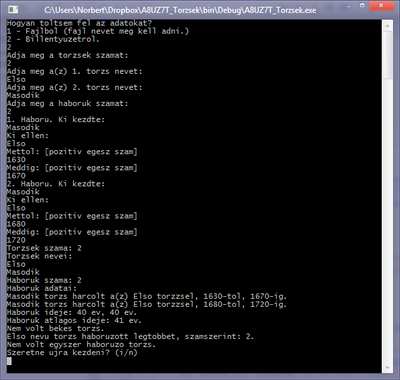
\includegraphics[scale=0.7]{billentyuzet}
\end{center}
Mintafutás fájból való beolvasás esetén:
\begin{center}
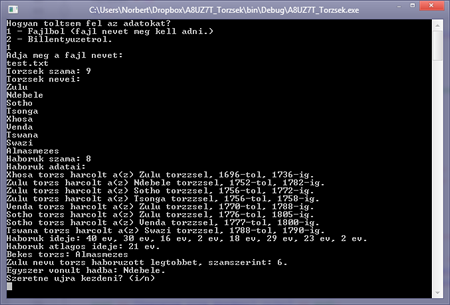
\includegraphics[scale=0.7]{fajlbol}
\end{center}
\pagebreak
\subsection{Hibalehetőségek}
A törzsek valamint háborúk száma legalább egy kell hogy legyen, és szöveg nem lehet. Ugyanez vonatkozik a háborúk idejére is. A háborúzók, valamint törzsek nevére nincs megkötés.\newline
\textbf{Mintafutás hibás adatok esetén:}
\begin{center}
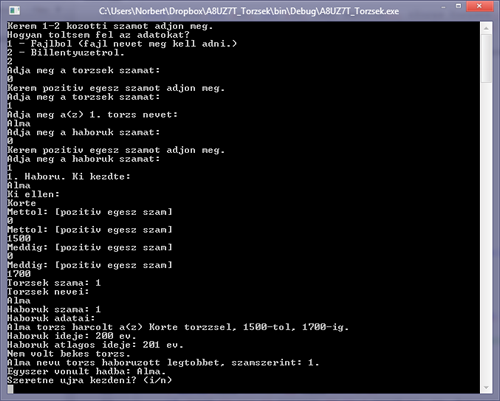
\includegraphics[scale=0.74]{hibas}
\end{center}
\mychapter{1}{Fejlesztői Dokumentáció}
\section{Feladat}
A jelenlegi Dél-Afrikai Köztársaság területén számos törzs élt, amikor a fehér gyarmatosítók
megjelentek. Közülük egyesek békében éltek, mások időről időre ellenséges viszonyba
keveredtek vagy éppen harcban álltak szomszédjaikkal. A háborúkat kezdőidő szerinti
sorrendben ismerjük a XVII., XVIII., XIX. századból.\newline

\vspace{1mm}

\begin{tabular}{rl}
\textbf{Sorszám} & \textbf{Feladat szövege} \\
D & Mennyi volt a háborúk átlagos ideje? \\
R & Volt békés törzs, és ha igen, akkor melyik? \\
BB & Melyik törzs háborúzott legtöbbször, és összesen mennyiszer? \\
TT & Volt egyszer hadba vonuló törzs, és ha igen, akkor melyik? \\
\end{tabular}
\section{Specifikáció}
Bemenet: tn, wn $\in$ $\mathbb{Z}$; Torzsek $\in$ tTorzs\textsuperscript{tn}, Haboruk $\in$ tWar\textsuperscript{wn}; tTorzs = nev, tWar = ki $\times$ kivel $\times$ mettol $\times$ meddig; ki, kivel, nev $\in$ S; mettol, meddig $\in$ $\mathbb{Z}$.
\newline
Előfeltétel: tn $>$ 0, $\forall$i(1 $\leq$ i $\leq$ tn): Torzsek\textsubscript{i}.nev $\not=$ '', Torzsek\textsubscript{i}.haboruk = 0,\newline
\-\hspace{1.85cm} wn $>$ 0, $\forall$i(1 $\leq$ i $\leq$ wn): Haboruk\textsubscript{i}.ki $\not=$ '',  Haboruk\textsubscript{i}.kivel $\not=$ '', Haboruk\textsubscript{i}.mettol $>$ 0, Haboruk\textsubscript{i}.meddig $>$ 0

\vspace{5mm}
\begin{Large}
\color{BlueB}{D feladat}
\end{Large}
\vspace{2mm}

Kimenet: atlag $\in$ $\mathbb{Z}$\newline
Utófeltétel: osszes =  $\sum\limits_{i=1}^{wn}$ Haboruk\textsubscript{i}.meddig - Haboruk\textsubscript{i}.mettol $\wedge$ atlag = $\frac{osszes}{wn}$

\vspace{5mm}
\begin{Large}
\color{BlueB}{R feladat}
\end{Large}
\vspace{2mm}

Kimenet: bekes $\in$ $\mathbb{S}$\newline
Utófeltétel: ind = $\exists$i (1 $\le$ i $\le$ tn): Torzsek\textsubscript{i}.haboruk=0 $\wedge$ bekes = Torzsek\textsubscript{ind}.nev

\vspace{5mm}
\begin{Large}
\color{BlueB}{BB feladat}
\end{Large}
\vspace{2mm}

Kimenet: Torzsek\textsubscript{max} $\in$ tTorzs\newline
Utófeltétel: 1 $\le$ max $\le$ tn $\wedge$ $\exists$i (1 $\le$ i $\le$ tn): Torzsek\textsubscript{max} $<$ Torzsek\textsubscript{i}

\vspace{5mm}
\begin{Large}
\color{BlueB}{TT feladat}
\end{Large}
\vspace{2mm}

Kimenet: bekes $\in$ $\mathbb{S}$\newline
Utófeltétel: ind = $\exists$i (1 $\le$ i $\le$ tn): Torzsek\textsubscript{i}.haboruk=1 $\wedge$ bekes = Torzsek\textsubscript{ind}.nev
\section{Megoldás}
\begin{Large}
\color{BlueB}{Programparaméterek}
\end{Large}
\vspace{5mm}

\begin{large}
\color{BlueB}{ \textit{Típus} }
\end{large}
\vspace{2mm}

tWar = Rekord (\newline
\-\hspace{2.3cm} ki: \-\hspace{0.88cm}Szöveg,\newline
\-\hspace{2.3cm} kivel:  \-\hspace{0.4cm}Szöveg,\newline
\-\hspace{2.3cm} mettol: \-\hspace{0.18cm}Egész,\newline
\-\hspace{2.3cm} meddig: Egész.\newline
)

tTorzs = Rekord (\newline
\-\hspace{2.3cm} nev: \-\hspace{0.88cm}Szöveg,\newline
\-\hspace{2.3cm} haboruk:  \-\hspace{0.1cm}Egész.\newline
)

\vspace{5mm}

\begin{large}
\color{BlueB}{ \textit{Változó} }
\end{large}
\vspace{2mm}

tn, wn: \-\hspace{0.88cm}Egész\newline
Torzsek: \-\hspace{0.6cm}Tömb[1..100: tTorzs]\newline
Haboruk: \-\hspace{0.46cm}Tömb[1..100: tWar]

\vspace{5mm}

\begin{large}
\color{BlueB}{ \textit{Programfelépítés} }
\end{large}
\vspace{2mm}

A program által használt modulok (és helyük):\newline
torzsekDRBBTT \-\hspace{4.88cm}- main.cpp.\newline
iostream, fstream, string, cstdlib, limits \-\hspace{1.15cm}- a C++ rendszer része.

\vspace{5mm}

\begin{large}
\color{BlueB}{ \textit{Függvénystruktúra} }
\end{large}
\vspace{10mm}


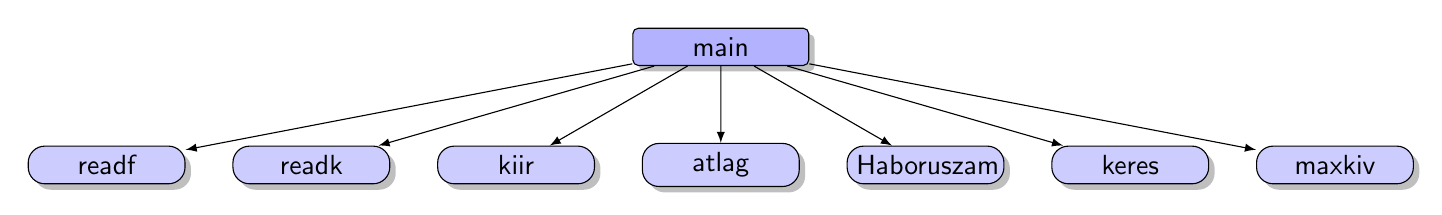
\begin{tikzpicture}[
  level 1/.style={sibling distance=26mm},
  edge from parent/.style={->,draw},
  >=latex]

% root of the the initial tree, level 1
\node[root] {main}
% The first level, as children of the initial tree
  child {node[level 2] (c1) {readf}}
  child {node[level 2] (c2) {readk}}
  child {node[level 2] (c3) {kiir}}
  child {node[level 2] (c4) {atlag}}
  child {node[level 2] (c5) {Haboruszam}}
  child {node[level 2] (c6) {keres}}
  child {node[level 2] (c7) {maxkiv}};


\end{tikzpicture}
\pagebreak

\begin{large}
\color{BlueB}{ \textit{Algoritmus} }
\end{large}
\vspace{2mm}

Az alprogramok algoritmusa a következő:

\vspace{2mm}
\color{white}{ \colorbox{Gray}{atlag(wn: Egész, Haboruk: tWar): Egész} }\newline
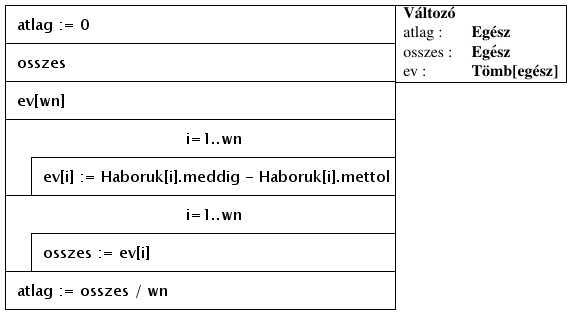
\includegraphics[scale=0.73]{atlag}

\colorbox{Gray}{keres(tn: Egész, Torzsek: tTorzs, int szam): Szöveg}\newline
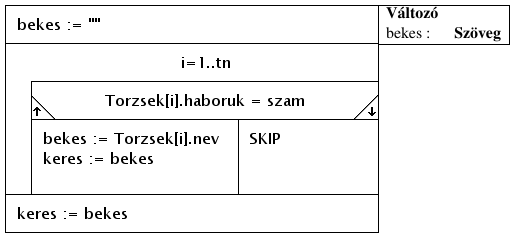
\includegraphics[scale=0.73]{keres}

\colorbox{Gray}{maxkiv(tn: Egész, Torzsek: tTorzs): tTorzs}\newline
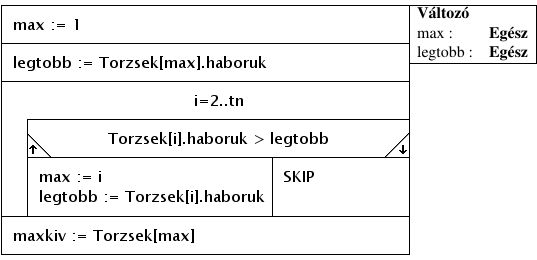
\includegraphics[scale=0.73]{max}

\pagebreak
\section{Tesztelés}
\begin{Large}
\color{BlueB}{Érvényes teszteset}
\end{Large}
\vspace{5mm}

\begin{table}[h]
\begin{tabularx}{\textwidth}{|l| X |l|}
\hline
\multicolumn{2}{|l|}{\textbf{Bemenet}} \\ \hline
\multicolumn{2}{|l|}{tn = 3}           \\ \hline
1                        & Zulu        \\ \hline
2                        & Sotho       \\ \hline
3                        & Venda       \\ \hline
\multicolumn{2}{|l|}{wn = 1}           \\ \hline
\multirow{4}{*}{1}       & Sotho       \\ \cline{2-2} 
                         & Venda       \\ \cline{2-2} 
                         & 1650        \\ \cline{2-2} 
                         & 1670        \\ \hline
\multicolumn{2}{|l|}{\textbf{Kimenet}}          \\ \hline
D                        & 20          \\ \hline
R                        & Zulu        \\ \hline
BB                       & Sotho       \\ \hline
TT                       & Sotho       \\ \hline
\end{tabularx}
\end{table}
\begin{Large}
\color{BlueB}{Érvénytelen teszteset}
\end{Large}
\vspace{5mm}

\begin{table}[h]
\begin{tabularx}{\textwidth}{|l| X |l|}
\hline
\multicolumn{2}{|l|}{\textbf{Bemenet}} \\ \hline
\multicolumn{2}{|l|}{tn = 0}           \\ \hline
\multicolumn{2}{|l|}{wn = 0}           \\ \hline
\multicolumn{2}{|l|}{\textbf{Kimenet}} \\ \hline
\multicolumn{1}{|c|}{D}       & -      \\ \hline
\multicolumn{1}{|c|}{R}       & -      \\ \hline
\multicolumn{1}{|c|}{BB}      & -      \\ \hline
\multicolumn{1}{|c|}{TT}      & -      \\ \hline
\end{tabularx}
\end{table}
\color{black}{ 
\section{Fejlesztési lehetőségek}
\begin{description}
  \item[Első] \hfill \\
  A törzsek tömbben lévő nevek összeegyeztetése a háború tömbben lévő ki/kivel nevű adataival.
  \item[Második] \hfill \\
  Az adatok dinamikus tömbben való tárolása, valamint újra futások esetén az előző adatok törlése.
\end{description}
}
\end{document}